\documentclass[11pt]{article}
\usepackage[margin=0.5in]{geometry}
\usepackage{mathtools,amssymb,scalerel}

\usepackage{graphicx} % Required for inserting images
\usepackage{hyperref}
\usepackage{listings}
\usepackage{tikz}
\lstset{breaklines=true}

\setlength{\parindent}{0cm}

\title{\LaTeX{} Intro Session}
\author{Jason Sinaga}
\date{Spring 2023}

\begin{document}
\maketitle

%%%%%%%%%%%%%%%%%%%%%%%%%%%%%%%%%%%%%%%%%%%%%%%%%%
%%%%% BASICS
%%%%%%%%%%%%%%%%%%%%%%%%%%%%%%%%%%%%%%%%%%%%%%%%%%
\section{Basics}
\LaTeX{} is a document preparation system. This will be especially helpful for Math 240 since you will be writing proofs on a regular basis. Since you'll be submitting your assignments through GradeScope, you want your work to be a legible as possible.
\vspace{3mm}

Note that it is always great to have paper as you work on your assignments. Reading \LaTeX{} commands is hard to understand.
\vspace{3mm}

Overleaf is a great tool for you to write .tex files. It can display your code on the left, your .pdf file on the right of the screen, and can also let you know of errors and can help you auto-fill commands. 
%%%%%%%%%%%%%%%%%%%%%%%%%%%%%%%%%%%%%%%%%%%%%%%%%%
%%%%% PREAMBLE
%%%%%%%%%%%%%%%%%%%%%%%%%%%%%%%%%%%%%%%%%%%%%%%%%%
\section{Preamble}
The preamble is the section of your \LaTeX{} document that tells the text editor what the file format you would use and what packages you want to use. This is what a simple preamble would look like.

\vspace{3mm}
\begin{figure}[htbp]
\centerline{\includegraphics[width=120mm]{Intro Session to LaTeX/Simple Preamble.png}}
\end{figure}
\vspace{3mm}

Since we are doing CS/Math 240, this kind of header would be more appropriate. Note that some features such as the margin and the removal of indentation is just personal preference.

\vspace{3mm}
\begin{figure}[htbp]
\centerline{\includegraphics[width=120mm]{Intro Session to LaTeX/Preamble.png}}
\end{figure}
\vspace{3mm}

Packages is a collection of extra commands that we can import so that we can use new the commands that we need for Mathematical symbols, notations, and operations.

\vspace{0mm}
\verb|\usepackage{mathtools,amssymb,scalerel}|
\vspace{0mm}

we would not be able to use Math symbols.
\pagebreak{}

We can also add a title, author, and date to our document. We can do so by writing these lines

\vspace{3mm}
\begin{figure}[htbp]
\centerline{\includegraphics[width=120mm]{Intro Session to LaTeX/Title.png}}
\end{figure}
\vspace{3mm}

It is important to write \verb|\maketitle| after \verb|\begin{document}| so that the title shows up on the document you are making.

%%%%%%%%%%%%%%%%%%%%%%%%%%%%%%%%%%%%%%%%%%%%%%%%%%
%%%%% COMMENTS
%%%%%%%%%%%%%%%%%%%%%%%%%%%%%%%%%%%%%%%%%%%%%%%%%%
\section{Comments}
Comments are a good way to organize your \LaTeX{} code so that it becomes more readable. These are texts that you can write on your workspace but do not show up on the document. To do this, use \verb|%Your comment here%|.

%%%%%%%%%%%%%%%%%%%%%%%%%%%%%%%%%%%%%%%%%%%%%%%%%%
%%%%% FORMATTING
%%%%%%%%%%%%%%%%%%%%%%%%%%%%%%%%%%%%%%%%%%%%%%%%%%
\section{Formatting}
\subsection{Text}
To modify text style, we can use these functions
\begin{enumerate}
    \item \verb|\textit{}| : \textit{This is italics}
    \item \verb|\textbf{}| : \textbf{This is boldface}
    \item \verb|\underline| : \underline{This is underline}
\end{enumerate}

We can also use these commands to modify the size
\vspace{3mm}

\begin{center}
\Large{This is large text. \verb|\Large{}|}
\vspace{0mm}

\huge{This is huge text. \verb|\huge{}|}
\end{center}

\subsection{Sections and subsections}
To divide your documents into parts, you can use the function \verb|\section{}|. Within those sections, you can even have subsections by using \verb|\subsection{}|
\vspace{3mm}

\subsection{Vertical space and organization}
When it comes to organizing your document, we cannot use enter to create vertical space. Instead, what you want to do is to use \verb|\vspace{3mm}| and enter the desired space between the curly braces. The amount of space desired is up to you.
\vspace{3mm}

It is important that when you use \verb|vspace{}|, you need to click enter afterwards so that you have the proper vertical space

\vspace{3mm}
\begin{figure}[htbp]
\centerline{\includegraphics[width=120mm]{Intro Session to LaTeX/Wrong Vspace.png}}
\caption{The wrong way to use vspace}
\end{figure}

\vspace{3mm}
\begin{figure}[htbp]
\centerline{\includegraphics[width=120mm]{Intro Session to LaTeX/Right Vspace.png}}
\caption{The right way to use vspace}
\end{figure}
\vspace{3mm}

If you want to separate pages manually, you can use \verb|\pagebreak{}|.

To write center-aligned text, you need to write the following

\begin{center}
This is a center-aligned text.
\end{center}

\subsection{Lists}
To make lists, you can do it in an ordered way or an unordered way. To do it in an unordered way, this is how you would do it. 

\vspace{3mm}
\begin{figure}[htbp]
\centerline{\includegraphics[width=120mm]{Intro Session to LaTeX/Unordered List.png}}
\end{figure}
\vspace{3mm}

This is how you would do it in an ordered way.

\vspace{3mm}
\begin{figure}[htbp]
\centerline{\includegraphics[width=120mm]{Intro Session to LaTeX/Ordered List.png}}
\end{figure}
\vspace{3mm}

%%%%%%%%%%%%%%%%%%%%%%%%%%%%%%%%%%%%%%%%%%%%%%%%%%
%%%%% MATH SYMBOLS
%%%%%%%%%%%%%%%%%%%%%%%%%%%%%%%%%%%%%%%%%%%%%%%%%%
\section{Math Symbols}
To use the Math symbols, we need to use the dollar signs. There are many Math symbols that you will use over the course of CS/Math 240. Here are some common symbols that you will use over the course.

\begin{itemize}
    \item \verb|\cap \cup \subseteq| : $\cap$ $\cup$ $\subseteq$
    \item \verb|\frac{numerator}{denominator}| : $\frac{x^2}{y^3}$
    \item \verb|\ge \le| : $\ge$ $\le$
    \item \verb|\sum_{n=1}^{\infty} 2^{-n}a| : $\sum_{n=1}^{\infty} 2^{-n}$ 
    \item \verb|\vee \wedge \neg| : $\vee \wedge \neg$
    \item \verb|\mathbb{Z} \mathbb{N} \mathbb{R}| : $\mathbb{Z}$ $\mathbb{N}$ $\mathbb{R}$
\end{itemize}

To use these symbols, we can use the \verb|$..$|. For example, the sentence \[A \cup{} (B \cap{} C)\]

We have to type it this way \verb|$A \cup{} (B \cap{} C)$|. 
\vspace{3mm}

Some symbols that appear on your keyboard may not appear on the document. For example, the \verb|< and >| symbols would end up as inverted question marks without the proper syntax. 
\vspace{3mm}

To circumvent this, we need to use this notation \verb|$>$| or \verb|$<$|. As a rule of thumb, all mathematical operators should be inside the dollar signs.
\vspace{3mm}

To have variables as exponents, you should use \verb|{}|. For example, to write $e^{x^{2}}$, the code needed is \verb|$e^{x^{2}}$|
\vspace{3mm}

When writing variables, it is recommended to use \verb|$$| to surround them so that they are stylized. Here is x and a stylized $x$.
\vspace{3mm}

We can also write subscripts on our variables. To do this, we can write \verb|$x_0$| to get $x_0$
\vspace{3mm}

If you are not sure of what command to use, the internet is your best friend.

%%%%%%%%%%%%%%%%%%%%%%%%%%%%%%%%%%%%%%%%%%%%%%%%%%
%%%%% MORE SYNTAX%%%%%%%%%%%%%%%%%%%%%%%%%%%%%%%%%%%%%%%%%%%%
\section{More Syntax}
When it comes to arithmetic, we can use the keyboard keys - x + /. However, we can use these commands for a more stylized notation.

\begin{itemize}
    \item \verb|+| : $+$
    \item \verb|-| : $-$
    \item \verb|\times| : $\times$
    \item \verb|\div| : $\div$
\end{itemize}

When writing mathematical expressions, you can fit in multiple Math commands within the \verb|$$| symbols. You do not need to 
\vspace{3mm}

For example, to write the expression

\[a_1 \le e^{x^{2}} + \frac{6!}{\sqrt{c}}\]

You can just write
\vspace{3mm}
\begin{center}
    \verb|$a_1 \le e^{x^{2}} + \frac{6!}{\sqrt{c}}$|
\end{center}

However, you need to be a bit more careful if you have a long Math expression that involves words in it. If you put in words within the dollar signs, the words will not be spaced out, and it will look something like this

\begin{center}
        $Let there be an expression a_1 \le e^{x^{2}} plus \frac{6!}{\sqrt{c}}$
\end{center}

To have a proper mathematical expression mixed with words, you need to put the dollar signs in the right place. By writing it like this

\begin{center}
    \verb |Let there be an expression $a_1 \le e^{x^{2}}$ plus $\frac{6!}{\sqrt{c}}$|
\end{center}

You will get this on your document.

\begin{center}
    Let there be an expression $a_1 \le e^{x^{2}}$ plus $\frac{6!}{\sqrt{c}}$ such that this becomes an example
\end{center}

Make sure that words are outside of the dollar signs.
\vspace{3mm}

When you want to write an equation that is emphasized and centered, you can use \verb|\[ \]| in place of \verb|$ $|. For example, by writing \verb|\[x^2 + 2x + 3 \ge 0\]|, you will get something like this.

\[x^2 + 2x + 3 \ge 0\]
\pagebreak{}

%%%%%%%%%%%%%%%%%%%%%%%%%%%%%%%%%%%%%%%%%%%%%%%%%%
%%%%% UPLOADING PICTURES
%%%%%%%%%%%%%%%%%%%%%%%%%%%%%%%%%%%%%%%%%%%%%%%%%%
\section{Pictures}

There may come a time that you need to upload a diagram to your document. To upload pictures, you can use this code

\vspace{3mm}
\begin{figure}[htbp]
    \centerline{\includegraphics[width=120mm]{Intro Session to LaTeX/Picture.png}}
\end{figure}
\vspace{3mm}

We can also add captions to our pictures by adding these lines of code.

\vspace{3mm}
\begin{figure}[htbp]
    \centerline{\includegraphics[width=120mm]{Intro Session to LaTeX/Picture Caption.png}}
\end{figure}
\vspace{3mm}

%%%%%%%%%%%%%%%%%%%%%%%%%%%%%%%%%%%%%%%%%%%%%%%%%%
%%%%% GRAPHS, TREES, STATE MACHINES
%%%%%%%%%%%%%%%%%%%%%%%%%%%%%%%%%%%%%%%%%%%%%%%%%%
\section{Graphs, Trees, State Machines}
In the later part of the course, you will be introduced to state machines, graphs, and trees. Technically, you could make a state machine from a graph. However, there is this great website that you can use to make a state machine. It can be found in section 9 (the section after this). 
\vspace{3mm}

In order to make graphs, you need to use the package \emph{tikz}. You also need to be able to picture the vertex placements on a cartesian plane or with some relative placement.
\vspace{3mm}

There are four kinds of graphs we can make.
\begin{itemize}
    \item Directed Graphs
    \item Undirected Graphs
    \item Weighted, directed graphs
    \item Weighted, undirected graphs
\end{itemize}
\vspace{3mm}
Generally, we can modify the color of the vertices and also add labels to each vertex. Let's look at the graphs we can make.

\pagebreak{}

\vspace{3mm}

\subsection{Directed graphs}

Directed graphs have arrows connecting one graph to another. 
The following code will generate a graph as follows.

\vspace{3mm}
\begin{figure}[htbp]
    \centerline{\includegraphics[width=140mm]{Intro Session to LaTeX/Digraph.png}}
\end{figure}
\vspace{3mm}

\begin{center}
    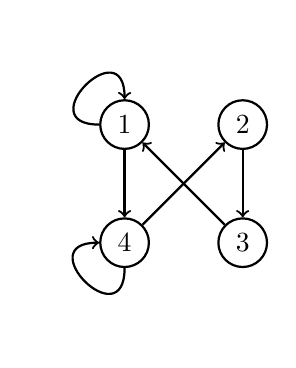
\begin{tikzpicture}[node distance={15mm}, main/.style = {draw, circle}, thick, ->] 
        \node[main] (1) {$1$}; 
        \node[main] (2) [right of=1] {$2$};
        \node[main] (3) [below of=2]{$3$};
        \node[main] (4) [below of=1]{$4$};
        \draw (1) to [out=180,in=90,looseness=5] (1); 
        \draw (1) -- (4); 
        \draw (2) -- (3);
        \draw (3) -- (1);
        \draw (4) -- (2);
        \draw (4) to [out=270,in=180,looseness=5] (4); 
    \end{tikzpicture} 
\end{center}

Notice that in the code section, there is \emph{main./style = {draw, circle}, thick, $->$}. This is a shortcut for us so that we don't need to retype the same style for numerous vertices/nodes.
\vspace{3mm}

Let's break apart the lines.
\vspace{3mm}

\verb|\node [main] (2) [right of=1] {$2$}|

\vspace{3mm}
After declaring a node/vertex, we need to put the style inside the first square brackets. Afterwards, we need to label the nodes. After labeling the node, the next square bracket is for placement. In this case, we are positioning the vertex relative to vertex 1. Lastly, we can label the vertex with a word or number. In this case, we are using a number.
\vspace{3mm}

\verb|\draw (1) to [out=180,in=90,looseness=5] (1);|

\vspace{3mm}
To create a line, we need to type draw. In the case where we need to create a line from a vertex to itself, we need to specify from which angle the arrow will go out and the angle the arrow will enter. Looseness influences how far the arrow will stretch away from the vertex before it returns.
\vspace{3mm}

\verb|\draw (4) -- (2);|

\vspace{3mm}
If there are no specific requirements of the arrows, we can just type -- to connect one vertex to another

\pagebreak{}

\subsection{Undirected graphs}
Undirected graphs are connected by lines. Let's look at the following code.

\vspace{3mm}
\begin{figure}[htbp]
    \centerline{\includegraphics[width=140mm]{Intro Session to LaTeX/Undigraph.png}}
\end{figure}
\vspace{3mm}

\begin{center}
    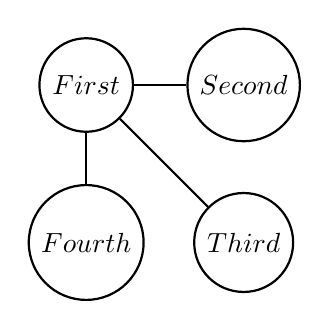
\begin{tikzpicture}[node distance={20mm}, main/.style = {draw, circle}, thick] 
        \node[main] (a) {$First$}; 
        \node[main] (b) [right of =a] {$Second$};
        \node[main] (c) [below of=b]{$Third$}; 
        \node[main] (d) [left of=c]{$Fourth$};
        %% Arrows
        \draw (a) -- (c);
        \draw (a) -- (b);
        \draw (a) -- (d);
    \end{tikzpicture} 
\end{center}

Let's break apart the lines.

\vspace{3mm}
\verb|\node[main] (b) [right of =a] {$Second$};|
\vspace{3mm}

As we can see from the code, we can see that this is not much different from the previous graph. In this case, we are using a word for our labels. Furthermore, the size of the vertex adjusts to the label in it. It is important to include the dollar sign when labelling a vertex/node.

\pagebreak{}

\subsection{Weighted, directed graphs}
This graph has labels on its arrows. Let's look at the code.
\vspace{3mm}

\vspace{3mm}
\begin{figure}[htbp]
    \centerline{\includegraphics[width=140mm]{Intro Session to LaTeX/Weighted digraph.png}}
\end{figure}
\vspace{3mm}

\begin{center}
    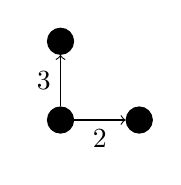
\begin{tikzpicture}
	\node[draw, circle, fill=black] (1) at ( 0, 0) {};
	\node[draw, circle, fill=black] (2) at ( 1, 0) {};
	\node[draw, circle, fill=black] (3) at ( 0, 1) {};

	\draw [->](1) -- (2) node[midway, below]		{2};
	\draw [->](1) -- (3) node[midway, left]		    {3};
    \end{tikzpicture}
\end{center}

Let's look at the lines more closely
\vspace{3mm}

\verb|\node[draw, circle, fill=black] (1) at ( 0, 0) {};|
\vspace{3mm}

On this line, we can see that we are using coordinates to place our vertices/nodes. This is another way of placement instead of using relative positions.
\vspace{3mm}

\verb|\draw [->](1) -- (2) node[midway, below]		{2};|
\vspace{3mm}

This line shows how we write our labels. In the square bracket after the connection between 1 and 2, we need to specify where exactly we want the label to be. In this case, midway is straightforward, and below tells us we want the weight to be under the line.

\pagebreak{}

\subsection{Weighted, undirected graphs}
This graph has labels on the edges connecting the vertices/nodes. Let's look at the code.

\vspace{3mm}
\begin{figure}[htbp]
    \centerline{\includegraphics[width=140mm]{Intro Session to LaTeX/Weighted undigraph.png}}
\end{figure}
\vspace{3mm}

\begin{center}
    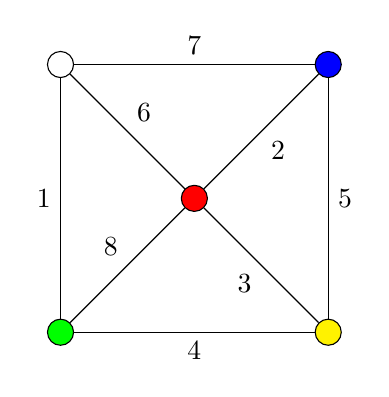
\begin{tikzpicture}
	\node[draw, circle, fill=red] (1) at ( 0, 0) {};
	\node[draw, circle, fill=blue] (2) at ( 1.7, 1.7) {};
	\node[draw, circle, fill=yellow] (3) at ( 1.7,-1.7) {};
	\node[draw, circle, fill=green] (4) at (-1.7,-1.7) {};
	\node[draw, circle, fill=white] (5) at (-1.7, 1.7) {};

	\draw (1) -- (2) node[midway, below right]		{2};
	\draw (1) -- (3) node[midway, below left]		{3};
	\draw (1) -- (4) node[midway, above left]		{8};
	\draw (1) -- (5) node[midway, above right]		{6};

	\draw (2) -- (3) node[midway, right]			{5};
	\draw (3) -- (4) node[midway, below]			{4};
	\draw (4) -- (5) node[midway, left]			    {1};
	\draw (5) -- (2) node[midway, above]			{7};
    \end{tikzpicture}
\end{center}

Let's break apart the lines.
\vspace{3mm}

\verb|\node[draw, circle, fill=white] (5) at (-1.7, 1.7) {};|
\vspace{3mm}

Here, we can change the color of vertices/nodes. This also works for nodes with names on it.

\pagebreak{}

%%%%%%%%%%%%%%%%%%%%%%%%%%%%%%%%%%%%%%%%%%%%%%%%%%
%%%%% GREAT EXTERNAL RESOURCES
%%%%%%%%%%%%%%%%%%%%%%%%%%%%%%%%%%%%%%%%%%%%%%%%%%
\section{Great external resources}
\begin{itemize}
    \item For making \textcolor{blue}{\href{https://madebyevan.com/fsm/}{state machines}}
    \item For finding the commands for \textcolor{blue}{\href{https://detexify.kirelabs.org/classify.html}{symbols}}
    \item For making \textcolor{blue}{\href{https://tikz.dev/tikz-graphs}{graphs}} 
\end{itemize}

%%%%%%%%%%%%%%%%%%%%%%%%%%%%%%%%%%%%%%%%%%%%%%%%%%
%%%%% NOW YOU TRY
%%%%%%%%%%%%%%%%%%%%%%%%%%%%%%%%%%%%%%%%%%%%%%%%%%
\section{Now you try}
Try to recreate the tutorial target \LaTeX{} document on your own. (It should be on the Canvas page of the class). Better yet, do it for your assignment.

\section{References}
begin{biblio}
\emph{List of LaTeX mathematical symbols - OeisWiki}. (n.d.). 
\vspace{0mm}

https://oeis.org/wiki/List\_of\_LaTeX\_mathematical\_symbols
\vspace{3mm}

\emph{Learn LaTeX in 30 minutes}. (n.d.). Overleaf, Online LaTeX Editor. 
\vspace{0mm}

https://www.overleaf.com/learn/latex/Learn\_LaTeX\_in\_30\_minutes\#Including\_title,\_author\_and\_date\_information

%%%%%%%%%%%%%%%%%%%%%%%%%%%%%%%%%%%%%%%%%%%%%%%%%%
%%%%% ACKNOWLEDGMENTS
%%%%%%%%%%%%%%%%%%%%%%%%%%%%%%%%%%%%%%%%%%%%%%%%%%
\section{Acknowledgments}
I would like to thank Professor Antoine Remond-Tiedrez for providing resources and .tex source files, and for reviewing this document. I would also like to thank the CS and Math Department of UW-Madison for allowing me to share this resource.

\end{document}

